\label{datasetAnalysis}
The data set we were working with consisted of pages which had been scraped\footnote{Web scraping is a method leveraged for the collecting of data from web pages with automated software rather than doing so manually. The software used for scraping loads a website, stores the desired data along with links to other pages and then loads those pages.} from the dark web utilising Ahmia \cite{ahmia} and stored in Elasticsearch (ES) \cite{elasticSearch} \cite{bcScraping}. This chapter describes the clear web, deep web, and the dark web, Elasticsearch, Ahmia, and the structure of the stored pages.

The Internet comprises networks from all over the world. The networks are connected and together they compose a global network. The Internet can be divided into the clear web, characterized in Section~\ref{clearWeb}, and the deep web, introduced in Section~\ref{deepWeb} \cite{internetStructure}.

\section{Clear web} \label{clearWeb}
The content of the clear web is indexed by search engines and is publicly accessible. The users are identified by their IP addresses and are usually not anonymous unless some privacy tools are used. The most used browsers worldwide according to market share are Chrome, Safari and Firefox \cite{browserMarketShare}. The size of the clear web is difficult to determine. However, it is estimated to contain about 5.93 billion pages as of March 2020 \cite{clearWebSize}.

\section{Deep web} \label{deepWeb}
The content of the deep web is not indexed by search engines and is not accessible publicly. Emails or medical information are examples of resources in the deep web. A user needs to be authorized to access this data. It is more problematic to measure the size of the deep web because of the fact the content is not indexed. There are not many sources depicting the size of the deep web. In one article from 2012 the size was estimated to be 4,000 to 5,000 times larger than the clear web \cite{deepWebSize}. 

A portion of the deep web is the \textit{dark web}, also called darknet. 
\subsection{Dark web} \label{darkWeb}
The dark web was designed to provide secure anonymity to users. It is therefore also leveraged for activities like accessing or publishing illegal or censored material, e.g. the Bible\footnote{The Bible is restricted in some countries, e.g. North Korea, or Iran \cite{illegalBible}.}, whistle-blower secrets, or child porn. It is also used for trading with illegal goods, such as drugs or guns. Another way to exploit the dark web is to offer or order illegal services, for instance money laundering, hacking or murder \cite{theDarkNet}. The onion router (Tor) or the Invisible Internet Project (I2P) are two of the networks composing the darknet. These networks are described more closely in Subsection \ref{tor} and Subsection \ref{I2P} respectively.

\subsection{Tor} \label{tor}
The Tor network \cite{torIntro} is accessible through the Tor browser or Tor proxy. Tor makes use of \textit{onion routing} (ORing) \cite{onionRouting}. ORing describes routing where each node, except for the originator and the target node, knows only its predecessor and successor. Determining the original source and target node is therefore difficult. ORing was introduced in the 1990s to ensure privacy. 

We now describe the establishment of an ORing connection. The visualization can be observed in Figure \ref{OREstablishment}. Public-key cryptography is used. The originator, in this case \textit{A}, chooses a list of nodes from which it creates a circuit between itself and the target node \textit{D}. \textit{A} creates a circuit consisting of itself and of nodes \textit{B}, \textit{C} and \textit{D}. \textit{A} creates a fixed-sized cell encrypted in layers using the respective public keys of the nodes in the circuit. The cell contains addresses of the circuit nodes and a different symmetric session key (SSK) for each node. \textit{A} stores the SSKs and sends this cell to \textit{B}. \textit{B} removes the outer layer of the cell using its private key in order to get the address of its successor, in this case \textit{C}, and the SSK assigned to \textit{B}. \textit{B} stores the SSK. \textit{B} cannot remove any additional layer because it lacks the private keys of the successive nodes. \textit{B} sends the cell to \textit{C}. \textit{C} removes another layer, stores the received SSK and, sends the cell to \textit{D}. \textit{D} removes the final layer and stores its SSK. Now \textit{D} is able to communicate with \textit{A} through \textit{B} and \textit{C} using symmetric cryptography. 

\begin{figure}[ht!]
  \centering
  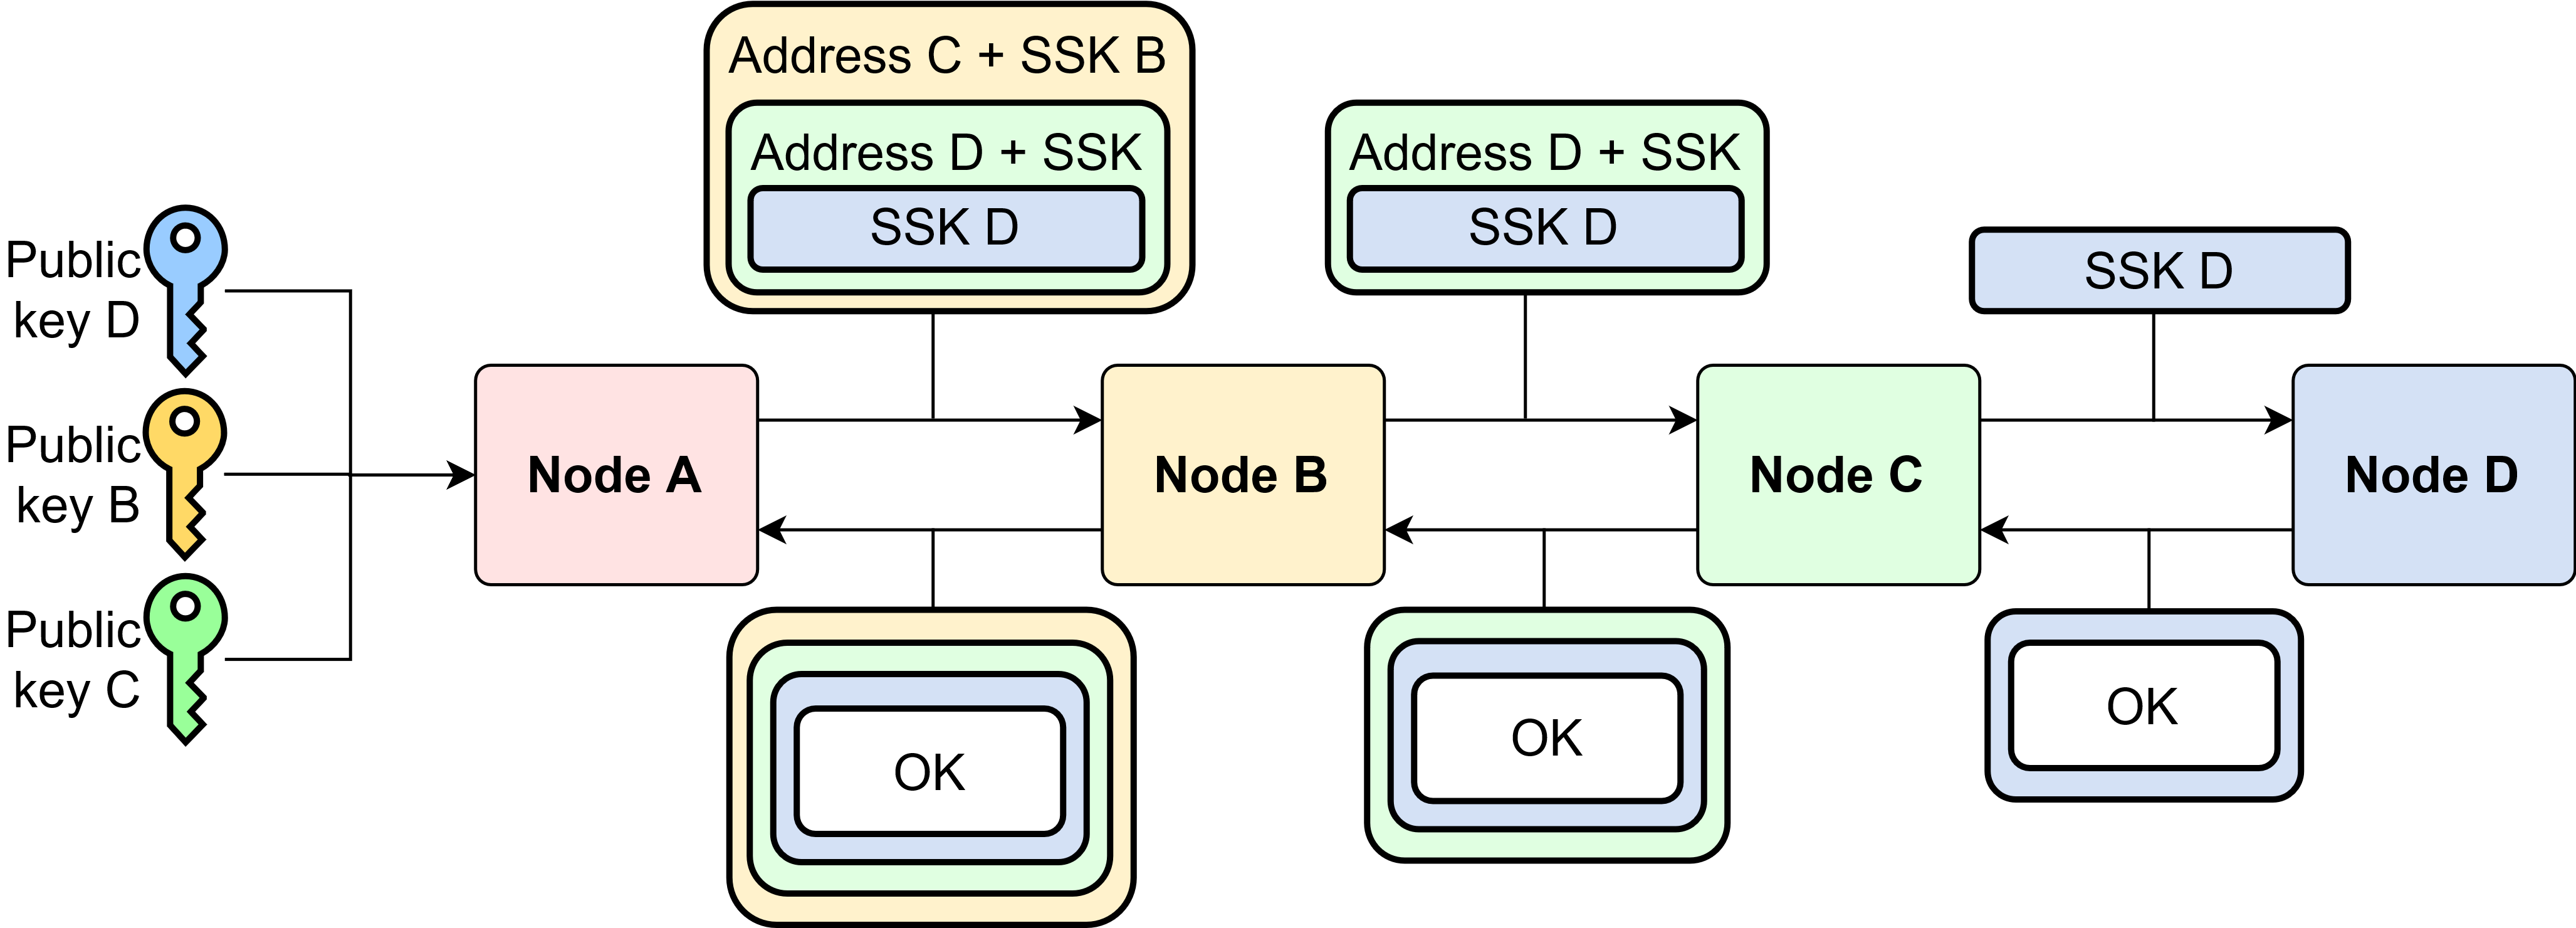
\includegraphics[width = \textwidth]{Images/OREstablishment.png}
  \caption{This is how a connection is established in ORing. The individual steps are described in Subsection \ref{tor}.}
  \label{OREstablishment}
\end{figure}

\begin{figure}[ht!]
  \centering
  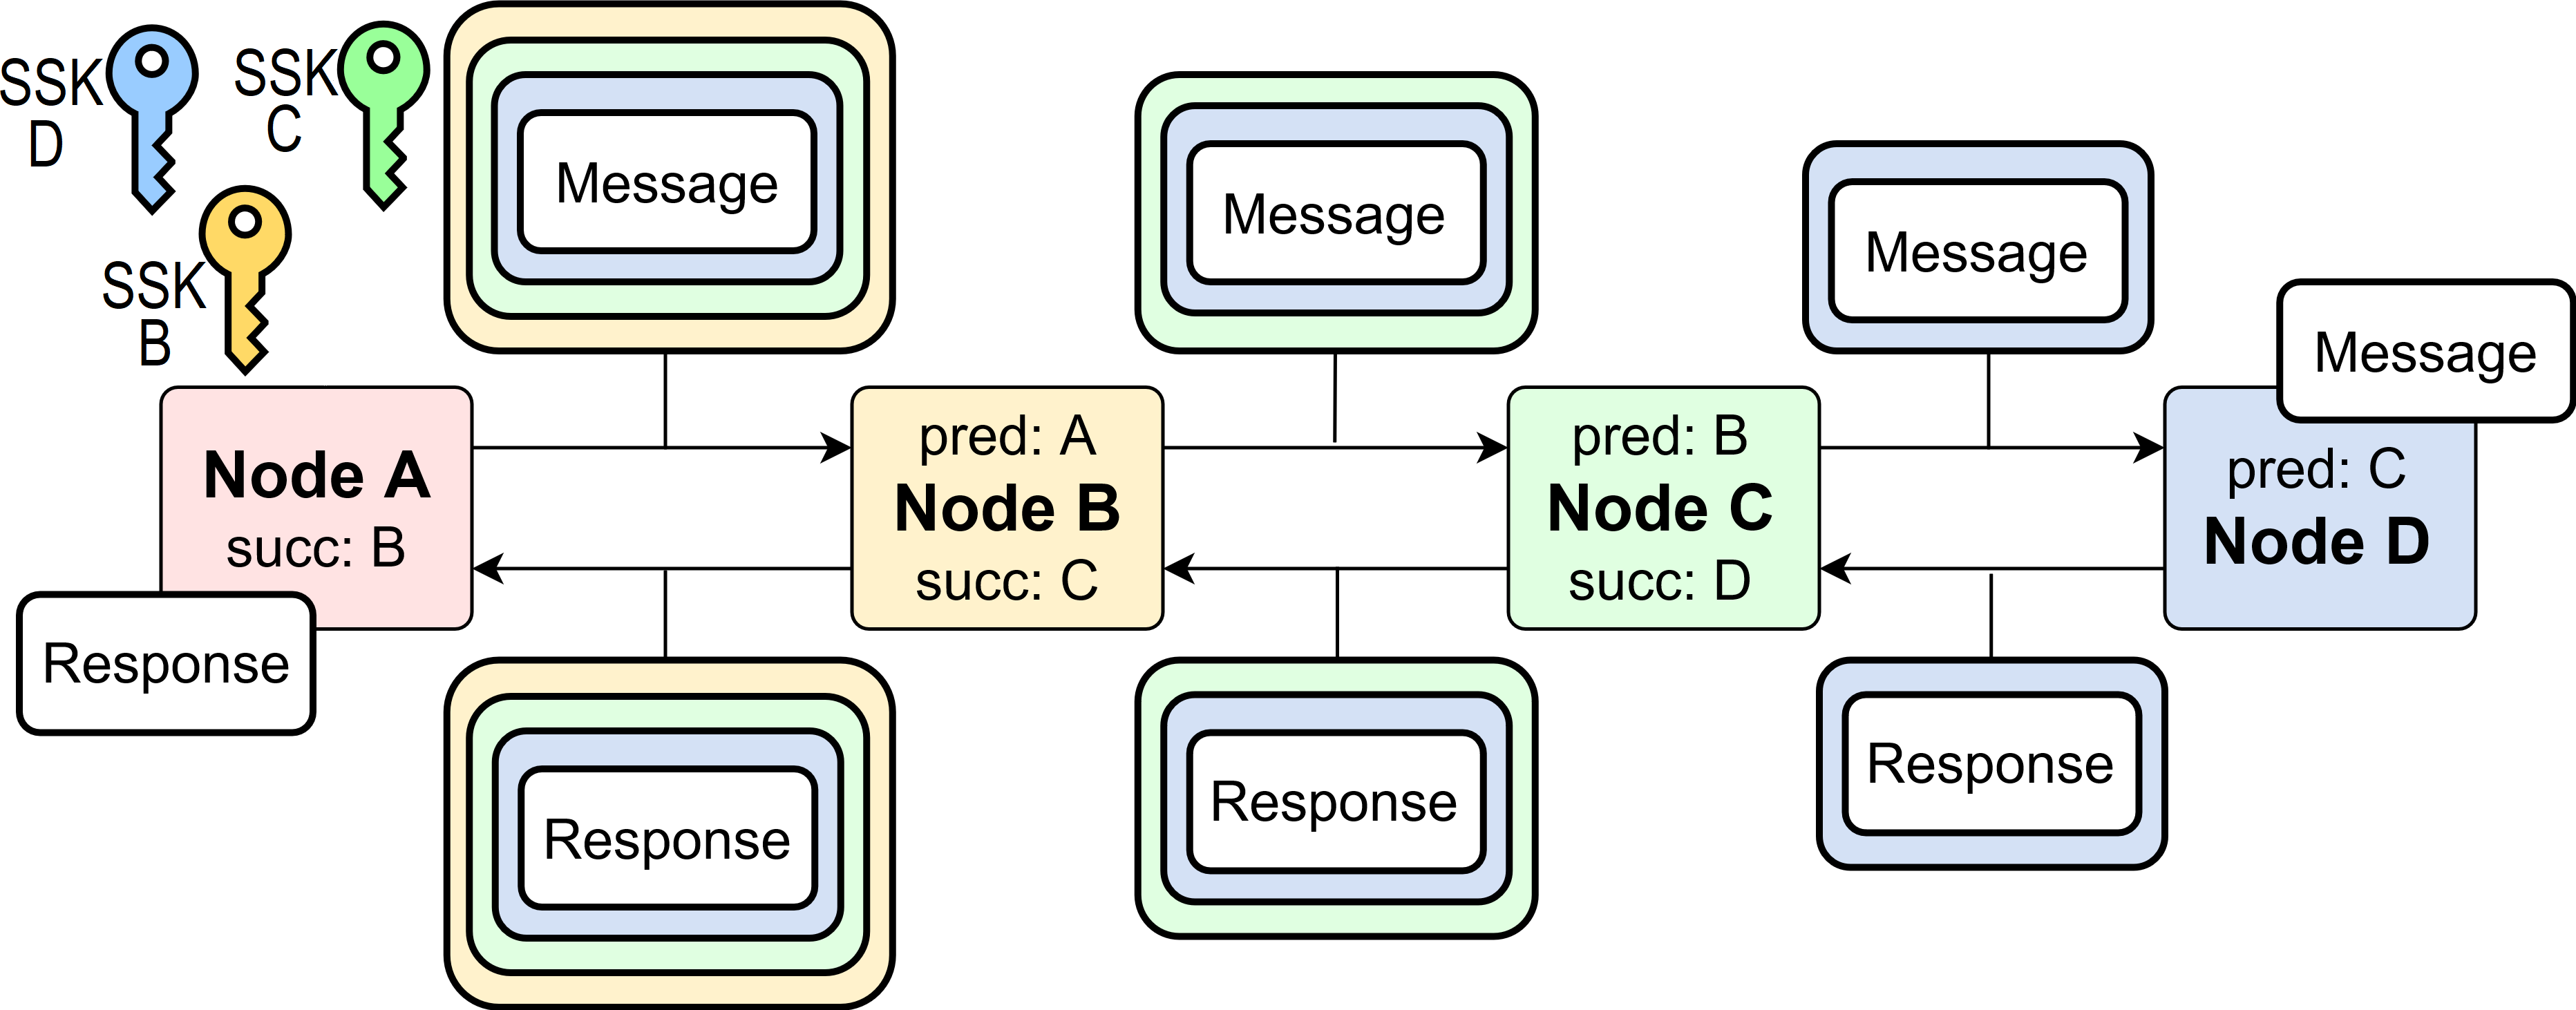
\includegraphics[width = \textwidth]{Images/ORCom.png}
  \caption{The communication between nodes in ORing is visualized in this image. The individual steps are described in Subsection \ref{tor}.}
  \label{ORCom}
\end{figure}

The communication in ORing is described in Figure \ref{ORCom}. Node \textit{A} encrypts a message using the symmetric keys of \textit{D}, \textit{C}, and \textit{B} in this order into a fixed-sized cell. It then sends the cell to \textit{B}. \textit{B} removes one layer of the cell, this time using its stored SSK. The message is sent to \textit{C} and \textit{D} in a similar manner. \textit{D} encrypts its response into a fixed-sized cell leveraging its stored SSK. The cell is sent to \textit{C}. \textit{C} encrypts the cell utilizing its SSK. The cell is sent to \textit{B} and \textit{A} in a similar manner. Node \textit{A} decrypts the cell using all three SSKs. 

\subsection{I2P} \label{I2P}
I2P \cite{i2pIntro} is another network of the dark web which anonymizes its traffic. It is accessible through the I2P browser. In contrast to Tor, communication in I2P is based on \textit{garlic routing} (GRing) \cite{garlicRouting}. GRing is described as an extension of ORing. The established tunnels between two nodes are unidirectional, meaning different tunnels are used for outgoing and incoming messages. Another difference from ORing is the bundling of messages. An individual message is called a \textit{clove}\footnote{Michael Freedman, who defined garlic routing, called cloves \textit{bulbs}.}. Each clove contains its own delivery instructions. These instructions are exposed at the target node. Cloves are bundled into a \text{garlic-message}. The bundling of cloves ensures more secure and efficient communication. 

Both exampled technologies provide anonymous access to the clear web as well as to the dark web. Both are open-source and free to use.

\section{The data set} \label{dataSet}
The dark web pages were acquired via web scraping. The scraped pages belonged to two different networks - I2P  and Tor. The total number of pages was 221,844. Of those pages 212,851 were Tor pages and 8,993 I2P pages. The total number of unique domains was 5,178 of which 4,912 were from the Tor network and 266 were from the I2P network. 

The fields of a page entry are described in the list~\ref{DWDataList}. Each description includes a concrete example from the database. Fields beginning with an underscore are assigned to every document implicitly.

\begin {description}
	\item[\_id \label{DWDataList}] is a unique identifier. For example\\ \textit{2d622b6fba6f203d790fedbb4f47963e2366c7fd}.
	\item[\_index] informs about the collection the document belongs to. For example \textit{tor}. 
	\item[\_type] determines the type of the document. For example \textit{\_doc}.
	\item[content] is the actual content of the page. For example \textit{Purple Kush – 10g – WackyWeed Menu    * Home   * Contact us   * About us }.
	\item[content\_type] describes the type of the content. For example \textit{text/html; charset=UTF-8}.
	\item[domain] of the url address. For example \textit{wacky2yx73r2bjys.onion}.
	\item[h1] is the text with the h1 style. For example \textit{Purple Kush – 10g}.
	\item[links] to other pages this page links to. For example \textit{\{\\
  "link": "http://wacky2yx73r2bjys.onion/",\\
  "link\_name": "Home"\\
\}}.
	\item[raw\_text] is similar to \textit{content}. It additionally may contain formatting elements such as \textit{\textbackslash n}. For example \textit{Purple Kush – 10g – WackyWeed Menu\textbackslash n\textbackslash n  * Home\textbackslash n  * Contact us\textbackslash n  * About us\textbackslash n }.
	\item[raw\_title] is similar to title. It additionally may contain formatting elements. For example \textit{Purple Kush – 10g – WackyWeed}
	\item[raw\_url] is the same as \textit{url}.
	\item[title] of the page. For example \textit{Purple Kush – 10g – WackyWeed}.
	\item[updated\_on] depicts the time when the document in the database was last updated. For example \textit{2019-10-22T19:41:09}.
	\item[url] address of the page. For example \\ \textit{http://wacky2yx73r2bjys.onion/?product=purple-kush-10g}.
\end{description}


\section{Ahmia} \label{ahmia}
Ahmia is a search engine mainly for domains of the Tor and I2P networks. Ahmia disposes of crawlers. The Ahmia crawlers were leveraged for the scraping of the pages. This is described in the bachelor's thesis by Juraj Noge \cite{bcScraping}. The mentioned thesis was being finished at the same time as this thesis.

\section{Elasticsearch}  \label{Elasticsearch}
The data collected from the dark web was stored in Elasticsearch. ES is a distributed, open source search engine \cite{elasticSearch} and offers a fast full-text search. Another benefit of ES are documentation and supported tools, such as Logstash \cite{logstash} for processing of data or Kibana \cite{kibana} for the visualization of data. ES can be used as a NoSQL database. Such a database consists of indexes, documents and fields as opposed to tables, rows and columns of SQL databases.  One of the advantages of NoSQL databases is scalability, therefore they are suited for big amounts of data. 